\documentclass{article}

\usepackage[margin=2.5cm,left=2cm,includefoot]{geometry}
\usepackage{graphicx}
\usepackage{float}
\usepackage[space]{grffile}
\usepackage{hyperref}
\usepackage[export]{adjustbox}
\usepackage{multicol}
\usepackage{caption}
\usepackage{hyperref}
\usepackage{listings}
\usepackage{vhistory}
\usepackage{titlesec}

\setcounter{secnumdepth}{4}

\titleformat{\paragraph}
{\normalfont\normalsize\bfseries}{\theparagraph}{1em}{}
\titlespacing*{\paragraph}
{0pt}{3.25ex plus 1ex minus .2ex}{1.5ex plus .2ex}

% Header and footer
\usepackage{fancyhdr}
\pagestyle{fancy}

\rhead{COS301}
\lhead{User Manual Document}
\fancyfoot[R]{Page \thepage}

\renewcommand{\headrulewidth}{2pt}
\renewcommand{\footrulewidth}{1pt}

\begin{document}

	\begin{titlepage}
		\begin{center}
			
\includegraphics[width=10cm]{images/UP.jpg}  \\
			[0.5cm]
			\huge{
			User Manual Document\\
			}
			
			\line(1,0){300}\\
			[0.2cm]
			\LARGE{Project: Insurance profiling from social media\\
			Client: RetroRabbit} \\
			\line(1,0){300}\\
			\LARGE{Team: Valknut Solutions}\\
			[1.0cm]
			\large{Version: 1.0}\\
			[1.0cm]
			\large
			{
			\begin{itemize}
				\item 13054903 - Charl Jansen van Vuuren 
				\item 10297902 - Bernhard Schuld      
				\item 13044924 - Kevin Heritage
				\item 13176545 - Quinton Weenink\\
			\end{itemize}
			}
			\textsc{\large}\\
		[3.0cm]
		\textsc{\large  Department of Computer Science}\\
		[0.5cm]
		\textsc{\large \today}\\
		\end{center}
	\end{titlepage}
	
	\cleardoublepage
	% Start of the revision history table
	\begin{versionhistory}
  		\vhEntry{1.0}{27.7.2016}{CJvV,KH,QW}{in progress}
	\end{versionhistory}	
	
	\cleardoublepage
	\tableofcontents
	\cleardoublepage
	
	\section{Introduction}
		This document contains information related to the use of the Insurance Profiling project that is being developed for RetroRabbit as part of the COS301 module at the University Of Pretoria.

	\section{References to other documentation}
		\begin{itemize}
			\item{Requirements specifications as per 29 July 2016}
			\item{Architecture Design as per 29 July 2016}
			\item{\href{https://www.facebook.com/business/a/lead-ads}{Facebook Lead adverts} as per 29 July 2016}
		\end{itemize}

	\section{Signing up your page}
		This section will cover the steps necessary for signing up your Facebook page in order for Facebook to send the data from the Lead Ads on your page through to the Insurance profiling server for processing.
		\begin{enumerate}
			\item Navigate to the website\\
			Open up the browser of your choice (Mozilla Firefox recommended) and navigate to the \href{https://insuranceprofiling.herokuapp.com}{Insurance Profiling} website.

			\item Sign up\\
			Click on the Sign Up button in the top right corner of the website\\
			\begin{figure}[H]
			  \centering
			      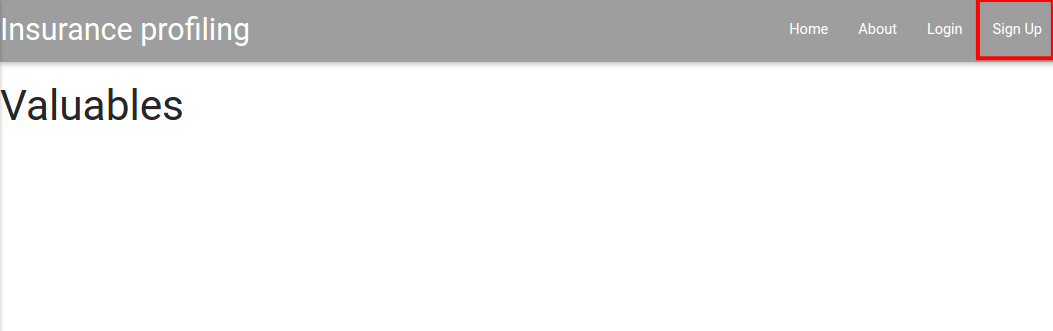
\includegraphics[width=\textwidth]{images/home_signup.png}
			  \caption{Home page indicating where to sign up}
			  \label{fig:homeSignup}
			\end{figure}

			\item Login with Facebook\\
			Once redirected click the button to Login with Facebook\\
			\begin{figure}[H]
			  \centering
			      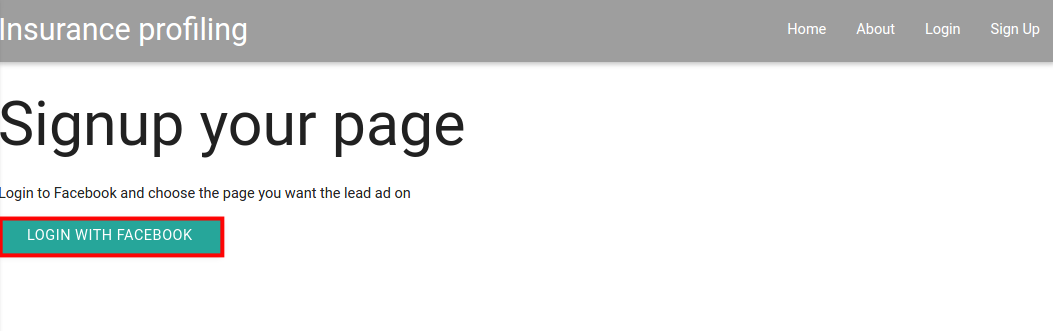
\includegraphics[width=\textwidth]{images/signup_login.png}
			  \caption{Button to click to login with Facebook}
			  \label{fig:signupLogin}
			\end{figure}
			When you have clicked the button a popup will appear requesting you to log into Facebook requesting permissions for the system to manage your pages.

		\item Selecting the page to manage\\
			Once the user has logged into their Facebook account with permission to manage their pages, a list of their pages will be displayed.\\
			Select the page that the system needs to manage.\\
			\begin{figure}[H]
			  \centering
			      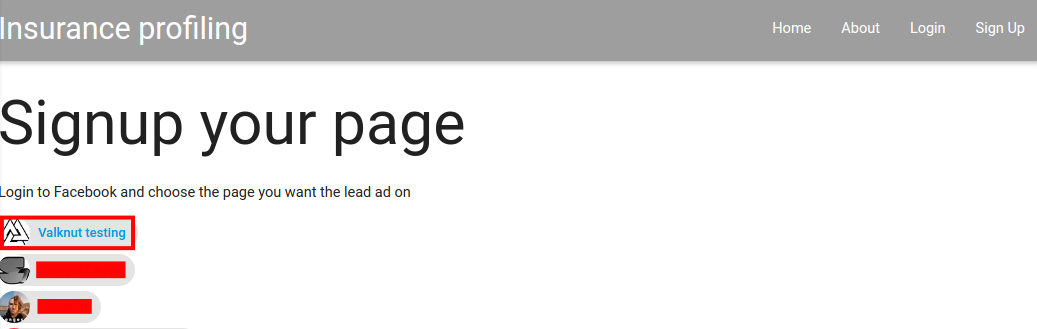
\includegraphics[width=\textwidth]{images/select_page.png}
			  \caption{Selecting the page to manage}
			  \label{fig:selectPage}
			\end{figure}
			When clicking on the page that the system should manage the user can create a lead ad.\\
			To create a lead ad user this Facebook references: \href{https://www.facebook.com/business/a/lead-ads}{Facebook Lead adverts}
		\end{enumerate}

\end{document}
